\documentclass[conference]{IEEEtran}

\ifCLASSINFOpdf
   \usepackage[pdftex]{graphicx}
   \graphicspath{{../pdf/}{../jpeg/}}
   \DeclareGraphicsExtensions{.pdf,.jpeg,.png}
\else
\fi

% correct bad hyphenation here
\hyphenation{op-tical net-works semi-conduc-tor}

% CUSTOM PACKAGES
\usepackage{amsmath}
\renewcommand{\arraystretch}{1.3}
\usepackage{etoolbox}
\apptocmd{\thebibliography}{\setlength{\itemsep}{0.6pt}}{}{}
\usepackage{url}
\usepackage{caption}
\usepackage{subcaption}
\usepackage{colortbl}
\usepackage{xcolor}
\definecolor{light-gray}{gray}{0.78}
\usepackage{epstopdf}
\usepackage{lettrine}
\usepackage{listings}


\begin{document}
\lstset{
  frame=none,
  xleftmargin=2pt,
  stepnumber=1,
  numbers=left,
  numbersep=5pt,
  numberstyle=\ttfamily\tiny\color[gray]{0.3},
  belowcaptionskip=\bigskipamount,
  captionpos=b,
  escapeinside={*'}{'*},
  language=haskell,
  tabsize=2,
  emphstyle={\bf},
  commentstyle=\it,
  stringstyle=\mdseries\rmfamily,
  showspaces=false,
  keywordstyle=\bfseries\rmfamily,
  columns=flexible,
  basicstyle=\small\sffamily,
  showstringspaces=false,
  morecomment=[l]\%,
}


\title{A Tool-chain for Instruction Set Architecture Design}

\author{
\IEEEauthorblockN{Alessandro de Gennaro}
\IEEEauthorblockA{School of Electrical and\\Electronic Engineering\\
Newcastle University\\
Newcastle upon Tyne, United Kingdom\\
Email: a.de-gennaro@ncl.ac.uk}
\and
\IEEEauthorblockN{Paulius Stankaitis}
\IEEEauthorblockA{School of Computing Science\\
Newcastle University\\
Newcastle upon Tyne, United Kingdom\\
Email: paulius.stankaitis@ncl.ac.uk}}

\maketitle

\begin{abstract}
Adopting a systematic approach for the design of a processor instruction set is
instrumental for tackling the complexity, which rules most of modern processors.

We present a tool-chain which follows the designer through all the phases of the
design, from the specification of instructions to the hardware synthesis of a
microcontroller. The flow is also meant to simplify the understanding of the
Instruction Set Architecture (ISA) reference manuals. Often, these documents are
semi-formal, hard to read and fully understand. We believe that designers will
benefit from a visual graph-based model, automatically derived from the ISA
specification, and customisable to fit different needs. Some of the tools have
already been developed and tested on ARMv6-M architecture, others yet need to be
fully implemented.

The design flow will be integrated inside the Workcraft framework. We also compare
the presented approach with the others available in the literature.
\end{abstract}

\IEEEpeerreviewmaketitle


\section{Introduction}
\label{sec:intro}
Technology progress allows industries to integrate always more transistors over the
same amount of area, following Moore's law. In turn, design complexity of these
systems progressively increases. This led research to be focused on raising the
level of abstraction of the languages used at the early-stages of design. This work
presents a design flow for an easier specification, visualisation, simulation,
customisation and hardware synthesis of instruction sets.

The consultation of an ISA reference manual (i.e. ARMv6-M \cite{armManual}) can be
a difficult and tedious operation. Anthony Fox, in his attempt to describe a model
of the ARMv7 instruction set, argues: ``official reference manuals are large,
stretching to many hundreds of pages - one can easily overlook subtle details or
become bogged down with ``uninteresting'' background information'' (\cite{armv7},
Section 1). And yet: ``official descriptions are semi-formal (ambiguous)''
(\cite{armv7}, Section 1). 

In the light of the above, a simple and formal way to specify and, more
specifically, visualise instruction sets is needed. A visual graph-based model can
help designers for a quicker comprehension of the processor. ISAs in fact provide a
software level description of the hardware itself. We use Conditional Partial Order
Graph (CPOG) \cite{cpog},\cite{andreyPhd} as the visualisation model. They can
efficiently represent concurrent and sequential behaviours, and already come with a
tested tool-kit for the customisation, encoding and hardware synthesis
(\cite{workcraft}, \cite{satEncoding}, \cite{acsd}).

We propose a new domain-specific language for ISA specification. The current
implementation is embedded in \textit{Haskell} This is a recent and extremely
flexible functional language, and provides predefined constructs and classes for
our purpose (i.e. monad class).

The article is organised as follows: Section \ref{sec:dsl} describes the framework
we have developed, and how this can be used to interact with all the steps of the 
design flow. Section \ref{sec:arm} presents a case-study: the ARMv6-M ISA and how this
can be converted into a more readable representation via the CPOG. 
And finally, Section \ref{sec:conclusion} summarises the achieved results, 
outlining the future research directions.

\subsection{Related work}

An attempt to use partial orders to describe the instructions of a complex hardware
structure can be found in \cite{maxPhd}. The author uses Conditional Partial Order
Graphs to visually describe the instructions of the Intel 8051 Microcontroller.
Yet, he used them for building an asynchronous controller and managing the internal
execution flow of the datapath elements. The manual construction of partial orders
is an error-prone process. Connecting all the operations taking into account their
dependencies and order is a complex task. This further inspired our research, and
led us to bridge this gap with an automated approach.

Regarding the language we chose to adopt, it is not difficult to find other cases
where functional languages have been used as a starting point for ISA
specification. In this direction, \cite{isaFunc} provides an interesting attempt to
build an infrastructure for instruction set development. The authors developed the
concepts of \textit{state} and \textit{transformations}. The former represents the
current state of the machine, which evolves over time according to the
transformations (instructions). \textit{F. Yuan and K. I. Eder} instead, created a
formal and hierarchical model, which can be refined for fitting the needs of a
particular ISA. This model (characterised in \cite{isaEventB}) is composed by 4
abstract layers. Each of these layers describes a particular aspect of the
instruction set. The deeper the designer explores this hierarchical representation,
the more refined will be the final system.

Another example can be found in \cite{armv7}. The authors here built a framework
which can be extended to tailor instruction sets. They use a monadic programming
style, based on three basic operations: \textit{return}, \textit{bind} and
\textit{parallel}. These are meant to mimic the flow of an entity (the hardware
system), which is always returned as a result of the execution of an instruction.
Instructions can be bound together either sequentially or in parallel. Here, the
case study used is the ARMv7, a widespread instruction set embedded by the 
Cortex-A8 processor. An additional example of how an ISA might be specified inside
a tool is present in \cite{isaXml}. Both the modules and the instructions here are
introduced via a xml-based language, fairly readable but not very flexible.

%------------------------------------------------

% Alex
\section{Domain Specific Language}
\label{sec:dsl}
% DSL introduction
The language used to describe the framework is Haskell \cite{haskell}. This is a 
functional language with high abstraction capabilities.
We followed the path, already explored in \cite{armv7}, implementing the \textit{monad class}
to build the infrastructure of the domain specific language (DSL).

The processor is seen as an entity composed by a combination of an internal and
external storage. Respectively, the former is represented by a set of registers,
while the latter by a memory that contains both instructions and data; in compliance with von
Newumann architecture. 

The processor executes instructions, that modify the state of the modelled machine.

$$P(Regs, Mem) \Rightarrow P'(Regs, Mem)$$

\noindent Every time the processor pulls off an instruction indeed, the state of the system
evolves into a new state $P'$ different from the previous one. Where either the registers and
the memory might be different. This approach is relatively similar to the processor
description in \cite{isaFunc}. Therefore, we are confident that the high degree of
abstraction obtained will allow to bidirectionally connect these two representations.

% Alex
\subsection{Structure of the framework}
\label{sec:struct}
% Description of the microprogram file
%  - how could be extended to fit the microprocessor model
%  - basic functions which each processor implements
%  - types used (Register - ComputationType - Address/Value)
%  - Monad class
%  - Processor seen as a Memory/register entity which evolves over time
What marks our approach is the high degree of flexibility and abstraction that can
extensively tailor every processor. The framework we present in this document is composed
by different layers (modelled in various and interconnected modules). Each of them plays 
an important role in the structure.

The module in charge of modelling the low-level hardware functions is named
\textit{basics}. Positioned at very bottom layer, this defines the ways through which the
memory elements can be accessed, the behaviour of the data-path components, 
as well as the monad basic functions: return and bind.

Furthermore, the types used in the structure are defined.
The registers and the memory are internally implemented with two maps of integer values.
The former can be accessed either via the name of a
special purpose register, or using the pattern $R \; Int$ (i.e. $R \; 5$, to point out the
fifth location of the register file). Memory is accessed via an integer type address instead.
Also immediate values are internally seen as integers. This approach is not
accurate. Some of the features - the bit length of the registers, or the
endianness of the data - are lost. Nonetheless, we aim at keeping a high degree of
abstraction, needed to interpret the model from several point of views (see Section
\ref{sec:func}).
Finally, ComputationType is defined. This is a flexible type in input to the
arithmetic logic unit (ALU), which can be modified according to the ISA
needs. As far as this unit is concerned in fact, different combinations of inputs can be
given to it: one single register for an increment/decrement operation, either two 
registers, or one register and an immediate for an ADD/SUB/MUL operation, and so on.
That is the main reason why this type needs to be scalable.

\textit{Microprogram} is the interface based on the low-level module just described.
In this, just a few operations, always present in a general purpose processor, are
implemented. The function for incrementing the program counter and fetching
the next instruction, the pop and push instructions, the interface methods for accessing
the registers and memory (internally modelled in the module basics).
In addition to the set of internal registers usually contained in a generic processor,
this module defines three registers more: the program counter, the instruction register and
the stack pointer.

\textit{ISA\_model} is the module where the user is supposed to introduce the custom 
instruction set architecture. Based on the bottom layers, this
module can be customised adding new special purpose registers and types for the ALU.
Most important, this will contain all the instructions one wants to include in a custom ISA. This will act as an interface for the software level simulation and will be taken into
account for the conversion towards other models and languages (Section \ref{sec:func}).

\textit{Main} is the module meant to the high-level software simulation, in here
all the instructions can be executed over the processor modelled. This might be useful
for having a first proof of a consistent architecture. The possible implementation errors
indeed, can be captured analysing the behaviour of the whole system.

\begin{figure}[ht!]
\begin{center}
	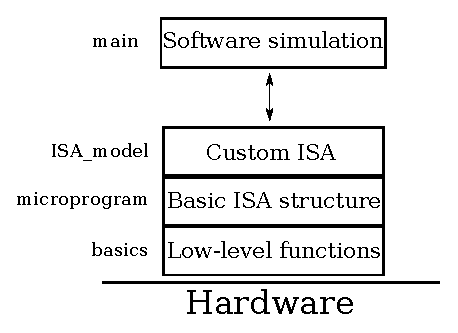
\includegraphics[scale=1]{IMG/structure.eps}
	\caption{Functional structure of the framework.}
	\label{fig:structure}
\end{center}
\end{figure}

In Figure \ref{fig:structure}, the whole structure of the framework is depicted, pinpointing 
on the interconnections between the modules described. 

In Section \ref{sec:arm} we will show how this framework has been implemented and extended
to model the ARMv6-M.

% Alex
\subsection{Functionalities \& interpretations}
\label{sec:func}
% Description of the tool-chain and of the ISA design flow
Our main goal with this article is to open the path towards an easier specification and
visualisation of instruction sets. Nonetheless, quite a few other interpretations can be
given to this work. The Domain Specific Language indeed, once used to model
a processor, can be potentially translated into other languages. In turn, they
can be progressively employed with the advantages and tools they come with. It is worth
mentioning that some of the functionalities discussed in this section have not been
implemented yet. Though, they will be part of our future work in this area (see Section
\ref{sec:frd}).

The ISA specification might be converted into Event-B language \cite{eventB}. This is a
formal technique used to analyse the model at the system level. It comes with some theorem
provers which are able to verify the consistency of the system, proving that there are 
no inconsistencies between instructions. This is an interesting feature itself, which could
be particularly useful when applied to instruction sets. It falls within the side of the
formal \textit{verification}.

\textit{Visualisation} and \textit{synthesis} are two other
interpretations which can be given to this framework, somehow connected to each other via
CPOG formalism. Even though Haskell provides readable and simple constructs, instruction
set specifications are intrinsically difficult to read and understand.
Capturing all the dependencies between every micro-operation within the instruction is
complex and, as already mentioned, error-prone. Reading the whole reference manual can take
long. In the light of the above, formal specification can be converted into partial orders,
a visual graph-based representation composed by nodes and arcs, much more readable either
than reference psuedo-code and Haskell statements.

\begin{figure}[ht!]
\begin{center}
	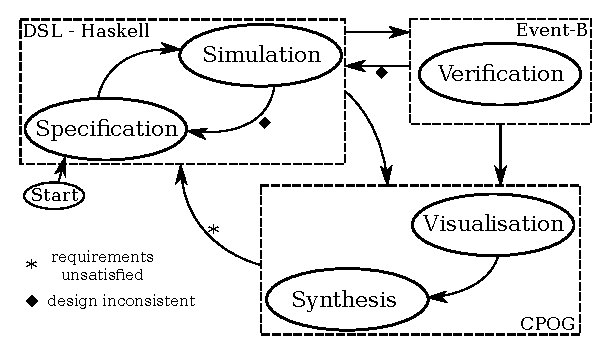
\includegraphics[width=\linewidth]{IMG/flow.eps}
	\caption{Design flow supported by the Haskell-based framework.}
	\label{fig:flow}
\end{center}
\end{figure}

This allows the user to employ the tool-chain around the conditional partial order
graphs. Either enabling the visual customisation of the dependencies of the instructions in 
\verb|Workcraft|, and the built-in synthesis tools available. A fairly
accurate measurement of the size of the final microcontroller for the processor control
unit can be automatically derived therefore, allowing the designer to come back at the
specification phase whether some of the requirements (area, power consumption) have not been
met.

A clearer picture of the whole design-flow is depicted in Figure \ref{fig:flow}.

%------------------------------------------------

% Paulius
\section{Case Study}
\label{sec:arm}
% Introduction of ARMv6-M ISA

% Paulius
\subsection{ARMv6-M}
% Description of the model in Haskell

% Alex & Paulius
\subsection{Towards readable specifications}
% Similarities between pseudo reference code and our model
% Show Partial order examples derived by hand
% Maybe an encoding example
Going towards a more readable specification was one of our main goal. As discussed in Section
\ref{sec:intro} in fact, often instruction set architecture reference document are hard to
read and fully understand. We believe that having a visual representation of the operations
which occur inside each instruction would make the understanding easier, yet quicker. That is
the main reason why we chose to adopt partial orders to represent the behaviour of
instructions. Each instruction can be analysed singularly. The behaviour can be isolated,
focusing on the causality of the operations to perform.

\begin{figure}[ht!]
\begin{center}
	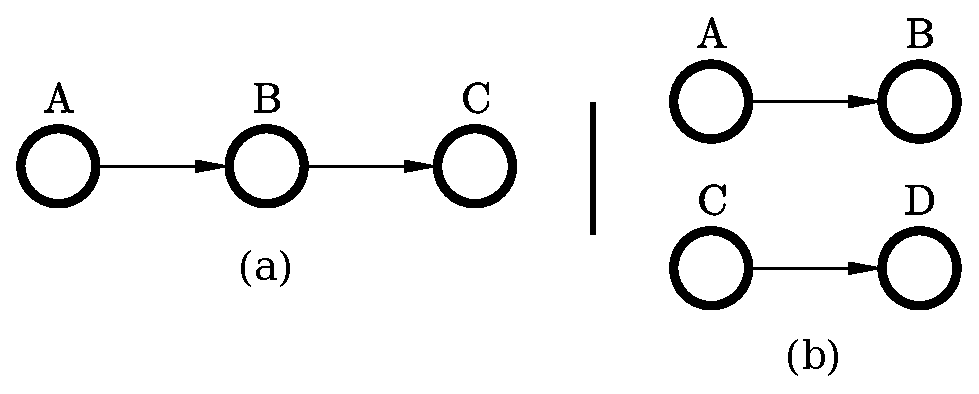
\includegraphics[scale=0.5]{IMG/pos.eps}
	\caption{Examples of sequential and concurrent behaviours.}
	\label{fig:pos}
\end{center}
\end{figure}

The capability of representing sequential and concurrent behaviours is instrumental for
modelling instructions. Partial orders address this requirement with the usage of nodes
($\bigcirc$) and dependencies ($\rightarrow$). Fig. \ref{fig:pos}(a) depicts a partial order
where the three operations are executed sequentially. Fig. \ref{fig:pos}(b) instead shows
four operations $\lbrace A,B,C,D \rbrace$ which can be executed with different orders. 
$\lbrace A,B \rbrace$ and $\lbrace C,D \rbrace$ are concurrent paths. A detail
description can be found in \cite{andreyPhd}.

In the light of the above, we are working on automating the conversion process from the
Haskell-based specification to partial orders. The tool will be able to analyse the
\textit{ISA\_module} file, capture the dependencies between the operations within each
instruction and build a partial order. 

Multiple levels of abstraction can be chosen for the conversion. Components such as the
arithmetic logic unit can be adopted for the execution of
different operations: i.e. addition, multiplication, shift, etc. One might want to represent
each single operation separately with a different node 
(trading off some readability with accuracy), or raise the
level of abstraction loosing the information about the actual operation.

\begin{figure}[ht!]
\begin{center}
	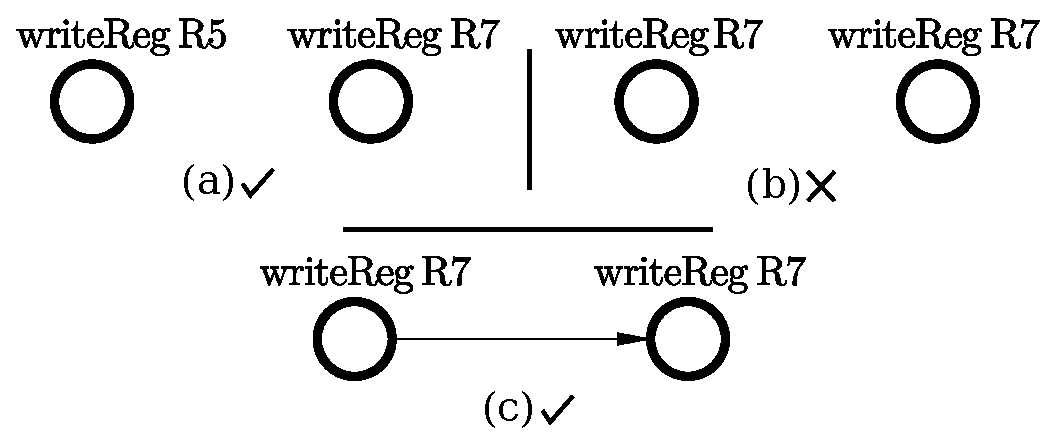
\includegraphics[width=\linewidth]{IMG/depPO.eps}
	\caption{Allowed and not allowed conversions.}
	\label{fig:depPO}
\end{center}
\end{figure}

The partial representation of the data, in some of the operations entailing registers and
memory access, represents another layer of abstraction which can be traded for readability.
This would allow the development of a more accurate model without overlapped register/memory
accesses. For instance, let us assume that the register file has got two different input
writing ports. This would allow two different registers to be written at the same time.
The destination of a writing operation should be taken into consideration therefore,
in order to avoid a simultaneous access at the same location of the register file.
(see Fig. \ref{fig:depPO}). The partial order in Fig. \ref{fig:depPO}(b) is not allowed
because the two writing mechanisms can be triggered concurrently.
A dependency should be inserted, as in the graph in Fig. \ref{fig:depPO}(c).

For easier the understanding of the reader, an example will be showed. In the Listing
\ref{lis:and} the specification of the AND (register) instruction (ARMv6-M ISA
\cite{armManual}) is depicted.\\

\begin{lstlisting}[caption="AND (register) instruction - Haskell-based specification",
frame=single, label=lis:and]
and_RegT1 :: ARMv6_M m => Register m -> Register m 
			 				 -> m ()
and_RegT1 rm rdn = do
    shifted <- alu (shlRegImm rm 0 apsr[29])
    result <- alu (andRegImm rdn shifted)
    writeRegister rdn result
    updateN result[31]
    updateZ result
    updateC carry
    incAndFetchInstruction
\end{lstlisting}

\noindent
This instruction can be automatically translated into the partial order in Figure
\ref{fig:andPO}. Every statement of the specification univocally corresponds to a node in the
graph. For instance, the one on sixth line correspond to the node named ``writeReg''.
The dependencies between the nodes are obtained by looking at the values which are needed for
the execution of each operation. For instance, the second ALU operation needs the value
called ``shifted'', computed during the first ALU operation. Therefore, the second action
depends on the first one.
``incAndFetchInstruction'' is a basic operation defined inside the module microprogram (see
Section \ref{sec:struct}). This is composed by three sequential operations, which are in this
case extracted and depicted in the partial order, for an increased accuracy.

\begin{figure}[ht!]
\begin{center}
	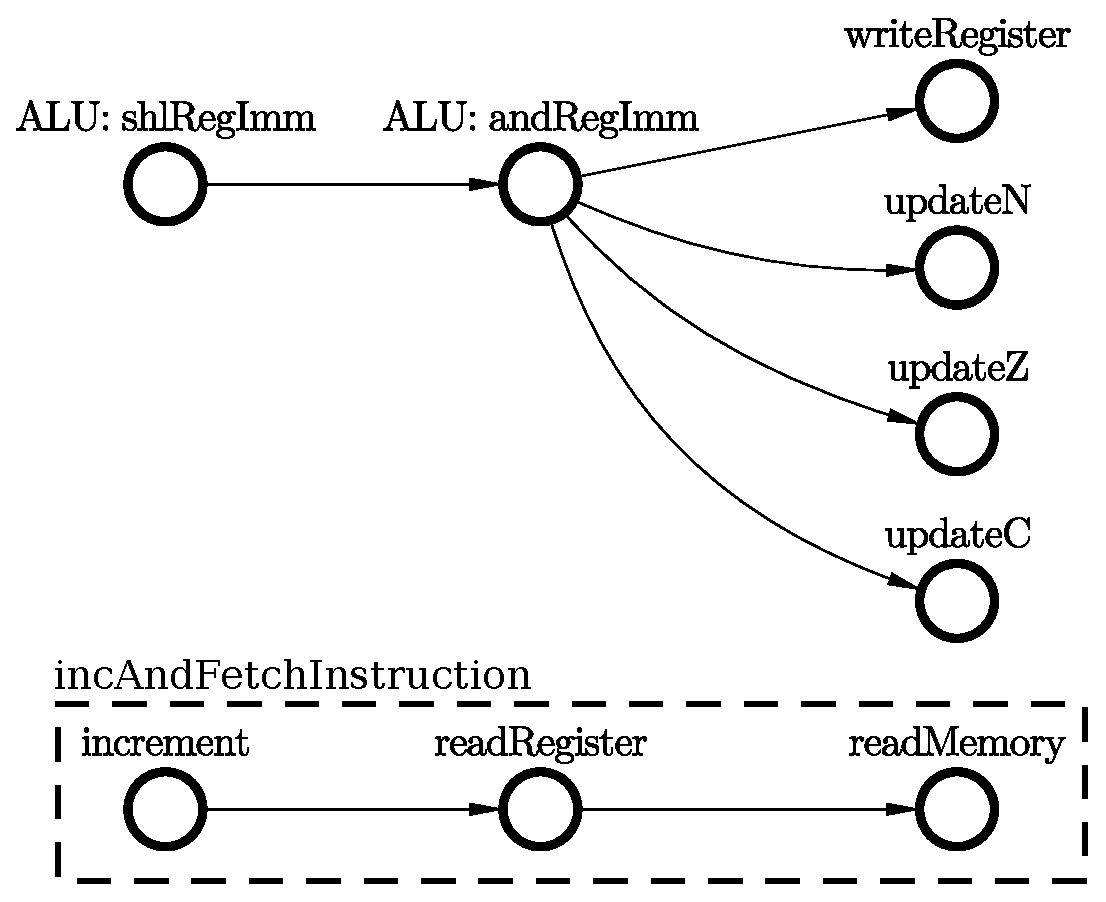
\includegraphics[width=\linewidth]{IMG/and_RegT1.eps}
	\caption{AND (register) instruction - ARMv6-M (\cite{armManual}, p.116)}
	\label{fig:andPO}
\end{center}
\end{figure}

The graph in Fig. \ref{fig:andPO} is more readable than the Haskell-based specification,
listed in Listing \ref{lis:and}. The dependencies between the various operations are
clearly expressed via arcs. In addition, the graph-based model provides a good degree
of fidelity; combined with the code-based specification it can lead to a good tradeoff
between readability and accuracy.

We did not have the time yet to implement the tool for the conversion.
The example showed along this section has been obtained by hand. Therefore, we reserve for a
future article the results and considerations related to the synthesis of the final
controller.

%------------------------------------------------

% Alex & Paulius
\section{Conclusion}
\label{sec:conclusion}
% Come up with some interesting conclusions

\subsection{Future research directions}
\label{sec:frd}
% future research direction

\noindent\textbf{Acknowledgements:} The authors would like to thank Dr. Andrey Mokhov for
helping with this work.

%------------------------------------------------

\begin{thebibliography}{1}

\bibitem{cpog}
	A. Mokhov, A. Yakovlev. \emph{``Conditional partial order graphs: Model,
	synthesis, and application''}. IEEE Transactions on Computers, Volume 59,
	Pages 1480-1493, November 2010.
	
\bibitem{andreyPhd}
	A. Mokhov. \emph{``Conditional Partial Order Graphs''}. Ph.D. Thesis,
	Newcastle University, September 2009.	

\bibitem{workcraft}
	I. Poliakov, D. Sokolov, A. Mokhov. \emph{``Workcraft: A static data flow
	structure editing, visualisation and analysis tool''}. Petri Nets and Other
	Models of Concurrency - ICATPN 2007. Pages 505-514, 2007.
	
\bibitem{satEncoding}
	A Mokhov, A Alekseyev, A Yakovlev. \emph{``Encoding of processor instruction
	sets with explicit concurrency control''}. Computers \& Digital Techniques,
	IET. Volume 5, Pages 427-439. November 2011.
	
\bibitem{acsd}
	A. de Gennaro, P. Stankaitis, A. Mokhov. \emph{``A Heuristic Algorithm for
	Deriving Compact Models of Processor Instruction Sets''}. 15th International
	Conference on Application of Concurrency to System Design (In Press). June
	24-26, 2015.

\bibitem{armv7}
	A. Fox, M. Myreen. \emph{``A Trustworthy Monadic Formalization of the ARMv7
	Instruction Set Architecture''}. Interactive Theorem Proving (ITP), pages
	243-258, 2010.	
	
\bibitem{isaEventB}
	F. Yuan, K. Eder. \emph{``A Generic Instruction Set Architecture Model in
	Event-B for Early Design Space Exploration''}. Technical Report CSTR-09-006,
	University of Bristol, September 2009.

\bibitem{isaFunc}
	T. A.Cook, E. Harcourt. \emph{``A Functional Specification Language for
	Instruction Set Architectures''}. Proceedings of the 1994 International
	Conference on Computer Languages. Publisher IEEE, pages 11-19. May 1994.
	
\bibitem{isaXml}
	A. Abbas, A. Ahmed, A. Ahmed, W. Uz Zaman Bajwa, A. Anwar, S. Abbasi. 
	\emph{``A retargetable tool-suite for the design of application specific
	instruction set processors using a machine description language''}. IEEE
	International Symposium on Circuits and Systems, 2002. Volume 1, pages 425-428.
	ISCAS 2002.
	
\bibitem{maxPhd}
	M. Rykunov. \emph{``Design of Asynchronous Microprocessor for Power
	Proportionality''}. Ph.D. Thesis, Newcastle University. Technical Report Series
	NCL-EEE-MICRO-TR-2013-182, December 2013.
	
\bibitem{armManual}
	ARM Ltd. \emph{``ARMv6-M Architecture Reference Manual''}. 
	ARM DDI 0419C (ID092410), 2010.
	
\bibitem{haskell}
	----. \emph{``Haskell 98 Language and Libraries The Revised Report''}. 
	Simon Peyton Jones (editor).
	
\bibitem{eventB}
	C. Métayer, J.-R. Abrial, L. Voisin. \emph{``Event-B Language''}. 
	Project IST-511599. $31^{st}$ May 2005
	
\end{thebibliography}

\end{document}